\begin{frame}[allowframebreaks]{Motivation}
	\textbf{\textcolor{blue}{Why Secret Sharing?}}
	\begin{itemize}
		\item Split a secret into \emph{shares} so that only authorized subsets can reconstruct it \cite{beimel2011secret}.
		\item Reduce single points of failure (key escrow, key backup, cloud storage, root keys).
		\item Foundation for threshold cryptography and secure multi-party computation.
		\item Used in practice for recovery and security hardening.
	\end{itemize}

	\begin{figure}
		\centering
		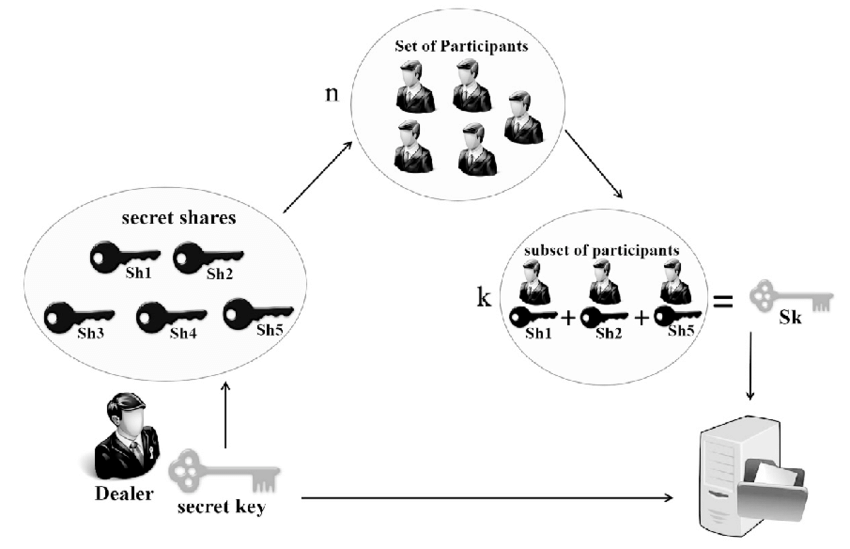
\includegraphics[scale=0.28]{fig/fig-threshold-secret-sharing.png}
		\caption{Threshold Secret Sharing intuition \cite{gutub2020}}
	\end{figure}
\end{frame}
